\documentclass[aspectratio=169]{beamer}
\usefonttheme[onlymath]{serif}
\usepackage[utf8]{inputenc}
\usepackage{graphicx} % Allows including images
\usepackage{booktabs} % Allows the use of \toprule, \midrule and \bottomrule in tables
\usepackage{subfigure}
\usepackage{subfiles}
\usepackage{url}
\usepackage{amssymb}
\usepackage{amsmath}
\usepackage{xcolor,colortbl}
\usepackage[backend=bibtex,sorting=none]{biblatex}
\usepackage[AutoFakeBold, AutoFakeSlant]{xeCJK}

\addbibresource{reference.bib} 

\definecolor{NJUPurple}{rgb}{0.41568, 0, 0.37255} 
\colorlet{LightNJUPurple}{white!60!NJUPurple}
\colorlet{SuperLightNJUPurple}{white!90!NJUPurple}

\usecolortheme[named=NJUPurple]{structure}

%Information to be included in the title page:
\title{深度强化学习中的迁移学习综述}
\author{\href{mailto:}{田鸿龙}}
\institute{LAMDA, Nanjing University}
\date{\today}

%Logo in every slide
\logo{%
  \makebox[0.98\paperwidth]{
    \href{https://www.nju.edu.cn}{
\includegraphics[height=0.75cm,keepaspectratio]{logos/nju_logo.jpg}}
    \hfill%
    \href{https://www.lamda.nju.edu.cn}{
\includegraphics[height=0.75cm,keepaspectratio]{logos/lamda_logo.png}}%
  }
}

\setbeamertemplate{blocks}[rounded][shadow=true]
\setbeamercolor{block title}{fg=white,bg=LightNJUPurple}
\setbeamercolor{block body}{fg=black,bg=SuperLightNJUPurple}
\setbeamerfont{title}{shape=\bfseries,size=\Large}
\setbeamerfont{author}{shape=\bfseries}

\makeatletter
\setbeamertemplate{title page}{%
  \vbox{}
  \vfill
  \vskip2cm%<- added
  \begingroup
    \centering
    \begin{beamercolorbox}[sep=8pt,center]{title}
      \usebeamerfont{title}\inserttitle\par%
      \ifx\insertsubtitle\@empty%
      \else%
        \vskip0.25em%
        {\usebeamerfont{subtitle}\usebeamercolor[fg]{subtitle}\insertsubtitle\par}%
      \fi%     
    \end{beamercolorbox}%
    \vskip1em\par
    \vfill%<- added
    \begin{beamercolorbox}[sep=8pt,center]{author}
      \usebeamerfont{author}\insertauthor
    \end{beamercolorbox}
    \vskip-0.2cm%<- changed
    \begin{beamercolorbox}[sep=8pt,center]{institute}
      \usebeamerfont{institute}\insertinstitute
    \end{beamercolorbox}
    \vfill%<- added
    \begin{beamercolorbox}[sep=8pt,center]{date}
      \usebeamerfont{date}\insertdate
    \end{beamercolorbox}%
    \vskip0.5cm%<- changed
  \endgroup
%  \vfill%<- removed
}
\makeatother


\AtBeginSection[]
{
  \begin{frame}
    \frametitle{Table of Contents}
  \tableofcontents[
        currentsection,
        currentsubsection,
        subsectionstyle=show/show/hide,
        sectionstyle=show/shaded
    ]
  \end{frame}
}

% you can comment to disable TOC before every subsection
\AtBeginSubsection[]
{
  \begin{frame}
    \frametitle{Table of Contents}
  \tableofcontents[
        currentsection,
        currentsubsection,
        sectionstyle=show/shaded,
        subsectionstyle=show/shaded/hide,
    ]
  \end{frame}
}
% shape, colour of item, nested item bullets in itemize only
\setbeamertemplate{itemize item}[circle] \setbeamercolor{itemize item}{fg=NJUPurple}
\setbeamertemplate{itemize subitem}[circle] \setbeamercolor{itemize subitem}{fg=LightNJUPurple}
\setbeamertemplate{itemize subsubitem}[circle] \setbeamercolor{itemize subsubitem}{fg=SuperLightNJUPurple}
% font size of nested and nested-within-nested bulltes in both itemize and enumerate
% options are \tiny, \small, \scriptsize, \normalsize, \footnotesize, \large, \Large, \LARGE, \huge and \Huge


\setbeamerfont{itemize/enumerate subbody}{size=\scriptsize} 
\setbeamerfont{itemize/enumerate subsubbody}{size=\scriptsize}


\newenvironment{splitframe}[5]
%[1] ==> 1 parameter passed through {}
%[2] ==> 2 parameters passed through {}{}
%[4] ==> 4 parameters passed through {}{}{}{}
    {
    \begin{frame}{#3}
    \begin{columns}
    \column{#1\linewidth}
    \centering
    #4
    \column{#2\linewidth}
    \centering
    #5
    \end{columns}
    \centering
    \vspace{\baselineskip} % adds one line space
    }
    %Inside the first pair of braces (ABOVE) is set what your new environment will do before the text within, then inside the second pair of braces (BELOW) declare what your new environment will do after the text. Note second pair can be empty braces too.
    {
    \end{frame}
    }

\begin{document}

\frame{\titlepage}

% no hyperlinks in logos except for titlepage
\logo{%
  \makebox[0.98\paperwidth]{
    
\includegraphics[height=0.75cm,keepaspectratio]{logos/nju_logo.jpg}
    \hfill%
    
\includegraphics[height=0.75cm,keepaspectratio]{logos/lamda_logo.png}%
  }
}

\section{Introduction}

\begin{frame}
  \frametitle{论文}

  \begin{figure}
    \centering
    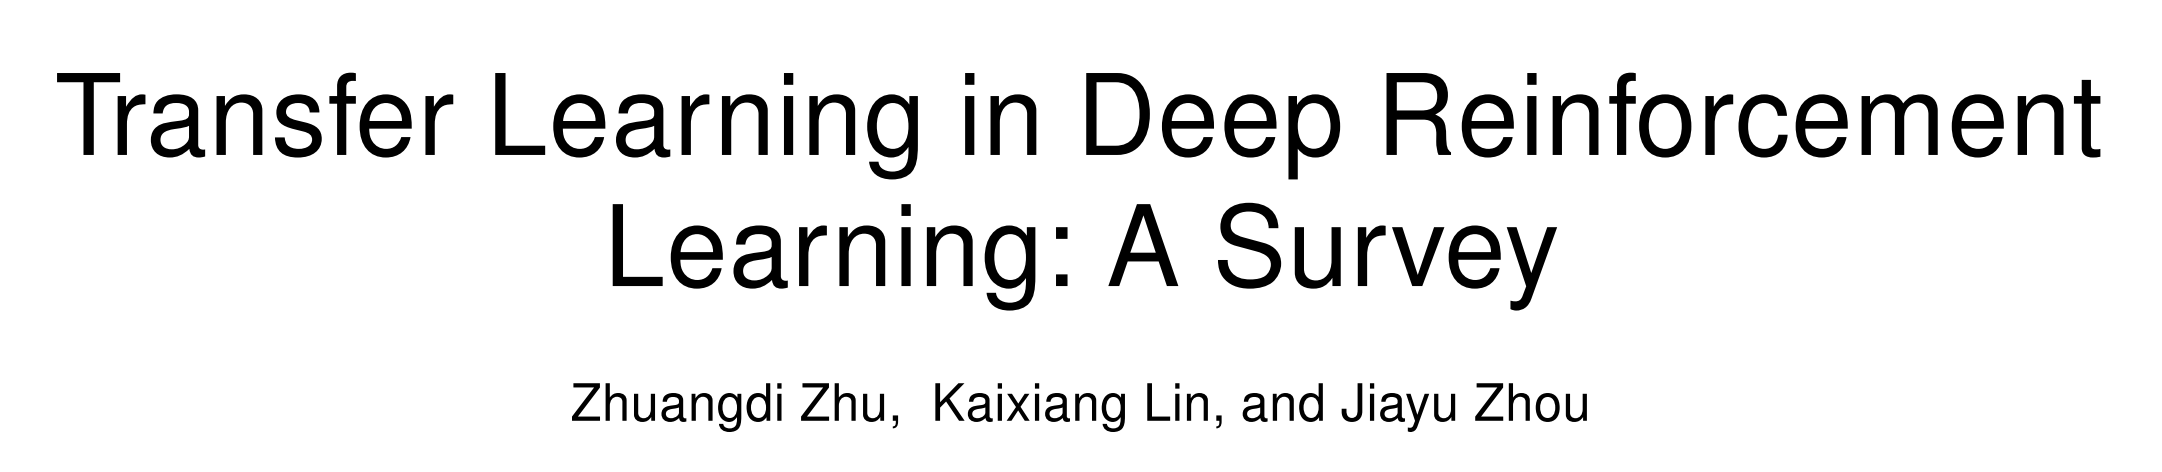
\includegraphics[width=1\textwidth]{imgs/paper.png}
  \end{figure}

\end{frame}

\begin{frame}
  \frametitle{Motivation}
强化学习面临相当多的问题,例如
\begin{itemize}
  \item partial observability
  \item sparsity and delay in the environment feedback
  \item high-dimensional observations and action spaces
  \item the cost of acquiring interaction samples can be prohibitive
  \item safety concerns in many real-world domains
  \item ...
\end{itemize}
因此在深度强化学习中利用之前的知识势在必行
\end{frame}

\begin{frame}
  \frametitle{TL in DRL}
  强化学习中的迁移学习更复杂,我们往往是将知识从一个MDP迁移到另一个MDP上,而这两个MDP可能具有很大差别。

  或者是将知识从专家迁移到智能体上,这也就是模仿学习。

  \begin{figure}
    \centering
    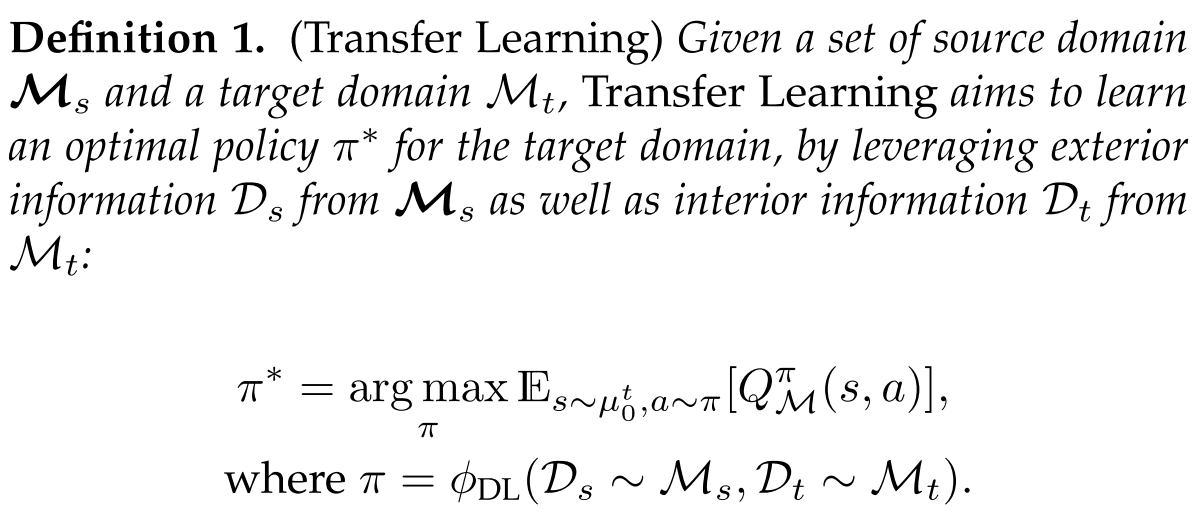
\includegraphics[width=0.8\textwidth]{imgs/TL_in_DRL_definition.png}
  \end{figure}
\end{frame}

\begin{frame}
  \frametitle{Related Topics}
  Imitation Learning
  \begin{itemize}
    \item  一些模仿学习算法只考虑了原域($D_s$)的知识,忽略了目标域($D_t$)的知识,例如行为克隆本质上是监督学习
    \item 另一些模仿学习算法既考虑了原域的知识,也考虑了目标域的知识,例如逆强化学习(和生成对抗模仿学习)
    \item 与Learning from Demonstrations (LfD)的区别:LfD发生在与RL环境的真实交互过程中,其目的是通过专家演示来实现有效的策略改进
  \end{itemize}
\end{frame}

\begin{frame}
  \frametitle{Related Topics(cont.)}
  Lifelong Learning
  \begin{itemize}
    \item  要求agent有能力学习在一个信息流中,多个时间上或者空间上相关的任务
    \item 要求学习一个新的任务之后不能忘掉过去的任务
    \item 获得终身学习的关键是在长期获得新信息和保留以前学到的知识以跨新任务转移之间进行权衡
    \item 终身学习往往比单纯的迁移学习更难
  \end{itemize}
\end{frame}

\begin{frame}
  \frametitle{Related Topics(cont.)}
  Hierarchical Reinforcement Learning (HRL)
  \begin{itemize}
    \item HRL往往对任务、动作和状态空间进行更高层次的抽象,从而形成更具有结构化的策略
    \item  因为策略结构可以通过抽象解耦,HRL促进了跨相似领域的知识转移
  \end{itemize}
\end{frame}

\begin{frame}
  \frametitle{Related Topics(cont.)}
  Multi-Agent Reinforcement Learning
  \begin{itemize}
    \item inter-agent transfer: reuse knowledge  received from com-munication with another agent, which has different sensors and (possibly) internal representations
    \item intra-agent transfer: reuse of knowledge generated by the agent in new tasks or domains
    \item see: A Survey on Transfer Learning for Multiagent Reinforcement Learning Systems
  \end{itemize}
\end{frame}

\section{Evaluating TL in DRL}

\begin{frame}
  \frametitle{Approach Categorization}
  What knowledge has been transferred?
  \begin{itemize}
    \item 即来自原域的知识的\textbf{形式}和\textbf{质量}
    \item 形式:例如一组专家经验、专家策略的行动概率分布,甚至可以是估计源/目标MDP中状态和动作对质量的潜在函数
    \item 知识形式和粒度上的差异影响了不同TL方法的内在逻辑
    \item 质量:oracle策略还是次优的人类演示
  \end{itemize}
\end{frame}

\begin{frame}
  \frametitle{Approach Categorization(cont.)}
  Where the transfer occurs?
  \begin{itemize}
    \item 有些TL方法适用于$M_s$和$M_t$相等的情况,而另一些方法则设计用于在不同MDP之间传递知识
    \item $M_s$和$M_t$之间的差异因任务而异
    \item 可能动作空间相同而状态空间不同,例如Atari
    \item 可能状态空间相同而动作空间不同,例如更改了机器人部件的型号
    \item 可能状态空间和动作空间都同,状态转移不同,例如Sim2Real
    \item 可能状态空间和动作空间都同,reward不同,例如不同的skills
  \end{itemize}
\end{frame}


\begin{frame}
  \frametitle{Approach Categorization(cont.)}
  How to transfer knowledge between source and target MPDs?
  \begin{itemize}
    \item 对Ms和Mt的相似性做了什么假设
    \item 从Ms到Mt的映射函数是预定义的还是自主生成的
    \item 学习过程的哪些组成部分,例如,学习策略π、价值函数V,甚至转换动力学T(对于基于模型的RL),可以从转移的知识中获益
    \item 这个映射的offline learning还是online learning
  \end{itemize}
\end{frame}


\begin{frame}
  \frametitle{Approach Categorization(cont.)}
  What goal to achieve for the transfer learning approach?
  \begin{itemize}
    \item 优化目标函数:在$D_t$上使用什么优化目标,例如为了让$D_s$的policy在新的MDP上探索,使用最大熵强化学习
    \item 评估指标:initial/convergence/episodic performance
  \end{itemize}
\end{frame}


\begin{frame}
  \frametitle{Approach Categorization(cont.)}
  How applicable a TL approach is?
  \begin{itemize}
    \item TL算法是policy-agnostic,还是依赖于某个set of algorithms
    \item 算法可以迁移哪些知识(见What knowledge has been transferred?)
    \item 算法在哪些“不同”上迁移(见Where the transfer occurs?)
  \end{itemize}
\end{frame}

\begin{frame}
  \frametitle{Approach Categorization(cont.)}
  What is the accessibility of the target MDP?
  \begin{itemize}
    \item 往往认为从源域访问知识的成本更低
    \item 由于目标MDP中的高采样成本,agent可能无法直接访问目标MDP,或者只能有非常有限的MDP交互
    \item 例如Sim2Real,需要在目标域考虑安全性,损耗等问题(例如那只伤痕累累的狗……)
  \end{itemize}
\end{frame}

\begin{frame}
  \frametitle{Approach Categorization(cont.)}
  How sample efficient the TL approach is?
  \begin{itemize}
    \item Zero-shot transfer:不需要在目标MDP交互
    \item Few-shot transfer:目标MDP交互很少
    \item Sample-efficient transfer:(多数算法处于这个级别)比在目标MDP直接训练效率更高
    \item 与目标MDP中从头开始的训练相比,TL方法使目标agent具有更好的初始性能(且在转移知识的指导下更快地收敛)  \end{itemize}
\end{frame}

\begin{frame}
  \frametitle{Potential Differences Among Tasks}
  \begin{itemize}
    \item $S$ (State-space)
    \item $A$ (Action-space)
    \item $R$ (Reward function)
    \item $T$ (Transition dynamics)
    \item $\mu_0$ (Initial states)
    \item $\tau$ (Trajectories)
  \end{itemize}
\end{frame}

\begin{frame}
  \frametitle{Evaluation metrics}
  \begin{itemize}
    \item Jumpstart Performance (jp): 初始表现
    \item Asymptotic Performance (ap): 最终表现
    \item Accumulated Rewards (ar): 积累reward,就是reward曲线下面积
    \item Time to Threshold (tt): 达到某个Threshold需要的时间
    \item Performance with Fixed Training Epochs(pe): 训练了固定轮数达到的表现
    \item Performance Sensitivity(ps): 算法受超参数的影响
  \end{itemize}
  
\end{frame}

\begin{frame}
  \frametitle{Evaluation metrics(cont.)}
  \begin{itemize}
    \item Transfer Ratio: with TL和Without TL下Asymptotic Performance的比值
    \item Required Knowledge Quantity (rkqt): 为了达到一定的性能阈值,迁移学习所需的知识数量,例如源任务的数量、专家策略的数量或用于实现知识转移的演示交互的数量
    \item Required Knowledge Quality (rkql): 为了达到一定的性能阈值,迁移学习所需的知识质量,例如TL方法是否依赖于源域中的近似oracle知识,或者给定次优知识,TL技术也能工作吗
  \end{itemize}
\end{frame}

\section{Transfer Learning Approaches}

\subsection{Reward Shaping}

\begin{frame}
  \frametitle{Reward Shaping}
  Reward Shaping利用先验知识重构目标MDP的奖赏分布,从而对agent的行为选择产生偏差

  $$
  \mathcal{M}=(\mathcal{S}, \mathcal{A}, \mathcal{T}, \gamma, \mathcal{R})) \rightarrow \mathcal{M}^{\prime}=\left(\mathcal{S}, \mathcal{A}, \mathcal{T}, \gamma, \mathcal{R}^{\prime}\right)
  $$
  
\end{frame}

\begin{frame}
  \frametitle{Reward Shaping(cont.)}
  Potential based Reward Shaping (PBRS)
  $$
  F\left(s, a, s^{\prime}\right)=\gamma \Phi\left(s^{\prime}\right)-\Phi(s)
  $$
  Potential Based state-action Advice (PBA)
  $$
  F\left(s, a, s^{\prime}, a^{\prime}\right)=\gamma \Phi\left(s^{\prime}, a^{\prime}\right)-\Phi(s, a)
  $$
  Dynamic Potential Based (DPB)
  $$
  F\left(s, t, s^{\prime}, t^{\prime}\right)=\gamma \Phi\left(s^{\prime}, t^{\prime}\right)-\Phi(s, t)
  $$

\end{frame}
\subsection{Learning from Demonstrations}

\begin{frame}
  \frametitle{LfD}
  传递的知识以外部演示的形式出现
  \begin{itemize}
    \item oracal策略
    \item 一个接近最优的专家策略
    \item 次优专家策略
  \end{itemize}
\end{frame}

\subsection{Policy Transfer}

\begin{frame}
  \frametitle{Policy Transfer}
  传递的知识是来自源任务的专家(教师)策略
  \begin{figure}
    \centering
    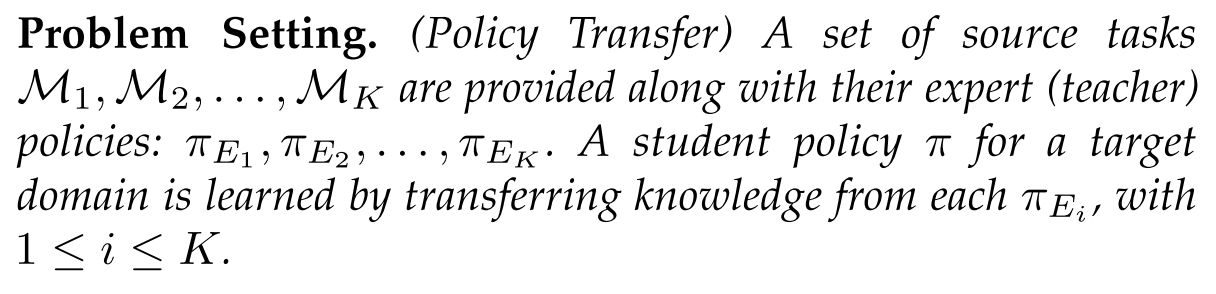
\includegraphics[width=0.8\textwidth]{imgs/policy_transfer.png}
  \end{figure}
\end{frame}

\begin{frame}
  \frametitle{Policy Transfer(cont.)}
  \begin{itemize}
    \item Transfer via Policy Distillation: 类似机器学习领域的知识蒸馏的概念,用若干个模型“教”一个新的模型
    \item Transfer via Policy Reuse: 直接重用源域的策略来构建目标域的策略
  \end{itemize}
\end{frame}

\subsection{Inter-Task Mapping}

\begin{frame}
  \frametitle{Inter-Task Mapping}
  在目标域和源域之间学习一个映射函数,主要考虑两个问题
  \begin{itemize}
    \item 映射函数适用于哪个领域
    \item 映射函数是如何被利用的
  \end{itemize}
  基本假设
  \begin{figure}
    \centering
    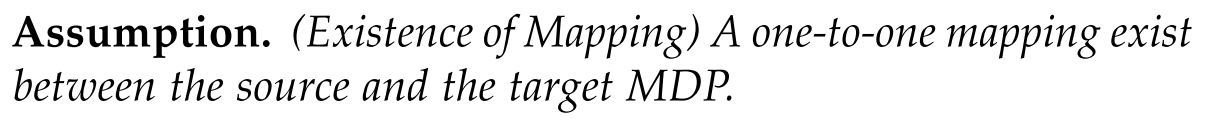
\includegraphics[width=0.8\textwidth]{imgs/existence_of_mapping.png}
  \end{figure}
\end{frame}

\subsection{Reusing Representations and Learning Disentangled Representations}

\begin{frame}
  \frametitle{Reusing Representations}
  \begin{itemize}
    \item 不需要学习任务之间显式映射
    \item 表示要么可以直接重用,要么存在任务不变的特征空间
    \item 知识就可以在特征空间上的任务之间传递
    \item 例如progressive network
  \end{itemize}
\end{frame}

\begin{frame}
  \frametitle{Learning Disentangled Representations}
  state space, action space, or even reward distribution space can be disentangled into independent, orthogonal sub-domains
  \begin{itemize}
    \item successor representation (SR)
    \item universal value function approximating (UVFA)
  \end{itemize}
\end{frame}

\end{document}

\end{document}